\documentclass[tikz,border=5pt]{standalone}
\usepackage{tikz}
\usetikzlibrary{positioning, arrows.meta, shapes.geometric, calc}

\begin{document}
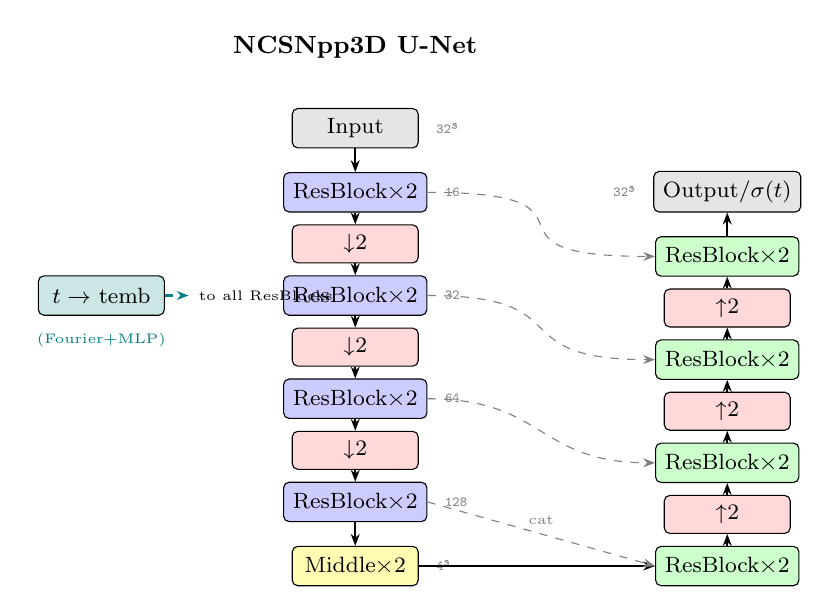
\begin{tikzpicture}[
    block/.style={rectangle, draw, minimum width=1.6cm, minimum height=0.5cm, rounded corners=2pt, font=\footnotesize},
    enc/.style={block, fill=blue!20},
    dec/.style={block, fill=green!20},
    mid/.style={block, fill=yellow!30},
    down/.style={block, fill=red!15, minimum height=0.35cm},
    up/.style={block, fill=red!15, minimum height=0.35cm},
    io/.style={block, fill=gray!20},
    temb/.style={block, fill=teal!20},
    arrow/.style={-{Stealth[length=1.5mm]}, thick},
    skip/.style={-{Stealth[length=1.5mm]}, dashed, gray},
    size/.style={font=\tiny\ttfamily, text=gray},
]

% Encoder column
\node[io] (in) {Input};
\node[size, right=0.1cm of in] {32³};

\node[enc, below=0.3cm of in] (e1) {ResBlock×2};
\node[size, right=0.1cm of e1] {16};
\node[down, below=0.15cm of e1] (d1) {↓2};

\node[enc, below=0.15cm of d1] (e2) {ResBlock×2};
\node[size, right=0.1cm of e2] {32};
\node[down, below=0.15cm of e2] (d2) {↓2};

\node[enc, below=0.15cm of d2] (e3) {ResBlock×2};
\node[size, right=0.1cm of e3] {64};
\node[down, below=0.15cm of e3] (d3) {↓2};

\node[enc, below=0.15cm of d3] (e4) {ResBlock×2};
\node[size, right=0.1cm of e4] {128};

% Middle
\node[mid, below=0.3cm of e4] (mid) {Middle×2};
\node[size, right=0.1cm of mid] {4³};

% Decoder column (to the right)
\node[dec, right=3cm of mid] (de4) {ResBlock×2};
\node[up, above=0.15cm of de4] (u3) {↑2};

\node[dec, above=0.15cm of u3] (de3) {ResBlock×2};
\node[up, above=0.15cm of de3] (u2) {↑2};

\node[dec, above=0.15cm of u2] (de2) {ResBlock×2};
\node[up, above=0.15cm of de2] (u1) {↑2};

\node[dec, above=0.15cm of u1] (de1) {ResBlock×2};

\node[io, above=0.3cm of de1] (out) {Output/$\sigma(t)$};
\node[size, left=0.1cm of out] {32³};

% Time embedding (left side)
\node[temb, left=1.5cm of e2] (temb) {$t \to$ temb};
\node[below=0.1cm of temb, font=\tiny, teal] {(Fourier+MLP)};

% Arrows - encoder
\draw[arrow] (in) -- (e1);
\draw[arrow] (e1) -- (d1);
\draw[arrow] (d1) -- (e2);
\draw[arrow] (e2) -- (d2);
\draw[arrow] (d2) -- (e3);
\draw[arrow] (e3) -- (d3);
\draw[arrow] (d3) -- (e4);
\draw[arrow] (e4) -- (mid);

% Arrows - middle to decoder
\draw[arrow] (mid) -- (de4);

% Arrows - decoder
\draw[arrow] (de4) -- (u3);
\draw[arrow] (u3) -- (de3);
\draw[arrow] (de3) -- (u2);
\draw[arrow] (u2) -- (de2);
\draw[arrow] (de2) -- (u1);
\draw[arrow] (u1) -- (de1);
\draw[arrow] (de1) -- (out);

% Skip connections
\draw[skip] (e4.east) -- node[above, font=\tiny] {cat} (de4.west);
\draw[skip] (e3.east) .. controls ++(1.5,0) and ++(-1.5,0) .. (de3.west);
\draw[skip] (e2.east) .. controls ++(2,0) and ++(-2,0) .. (de2.west);
\draw[skip] (e1.east) .. controls ++(2.5,0) and ++(-2.5,0) .. (de1.west);

% Time embedding arrow
\draw[arrow, teal, dashed] (temb.east) -- ++(0.3,0) node[right, font=\tiny, black] {to all ResBlocks};

% Title
\node[above=0.5cm of in, font=\small\bfseries] {NCSNpp3D U-Net};

\end{tikzpicture}
\end{document}
